% ====================================================================
% Tabelas e figuras de benchmark -- GERADO automaticamente.
% Recorte oficial: Random Forest, SVM, CCT, AST, Res2Net, Conformer,
% RawNet2, AASIST, RawGAT-ST, WavLM Original e HuBERT Original.
% Nao editar a mao; regenerar com:
%   python scripts/reporting/consolidate_results.py <runs...> --prefer-last --copy-to data/results/paper/figures
%   python scripts/reporting/update_tcc_latex.py
% ====================================================================

\begin{table}[ht]
\centering
\caption{Resultados consolidados no conjunto de teste limpo.}
\label{tab:resultados_consolidados}
\resizebox{\textwidth}{!}{%
\begin{tabular}{lcccccccc}
\hline
Modelo & Acur. & EER & $t$-DCF$^\ast$ & AUC & F1 & Lat.\,(ms) & Treino & Status \\
\hline
        Random Forest & 91,53\% & 6,95\% & 0,1966 & 0,984 & 91,22\% & 56,43 & CV+fit & \textcolor{successgreen}{OK} \\
        SVM & 93,20\% & 6,95\% & 0,1457 & 0,973 & 92,85\% & 0,90 & CV+fit & \textcolor{successgreen}{OK} \\
        CCT & 99,57\% & 0,43\% & 0,0085 & 1,000 & 99,57\% & 31,83 & 100 & \textcolor{successgreen}{OK} \\
        AST & 99,71\% & 0,14\% & 0,0041 & 0,999 & 99,71\% & 44,46 & 100 & \textcolor{successgreen}{OK} \\
        Res2Net & 97,76\% & 2,17\% & 0,0513 & 0,998 & 97,74\% & 46,41 & 100 & \textcolor{successgreen}{OK} \\
        Conformer & 98,91\% & 0,29\% & 0,0054 & 1,000 & 98,91\% & 50,46 & 100 & \textcolor{successgreen}{OK} \\
        RawNet2 & 95,88\% & 3,18\% & 0,0762 & 0,997 & 95,72\% & 90,08 & 100 & \textcolor{successgreen}{OK} \\
        AASIST & 94,72\% & 2,60\% & 0,0721 & 0,989 & 94,93\% & 53,38 & 100 & \textcolor{successgreen}{OK} \\
        RawGAT-ST & 87,55\% & 11,87\% & 0,3149 & 0,947 & 88,55\% & 54,45 & 100 & \textcolor{successgreen}{OK} \\
        WavLM Original & 96,09\% & 3,62\% & 0,0792 & 0,996 & 96,12\% & 15,77 & 100 & \textcolor{successgreen}{OK} \\
        HuBERT Original & 93,92\% & 5,93\% & 0,1308 & 0,987 & 93,93\% & 15,98 & 100 & \textcolor{successgreen}{OK} \\
\hline
\end{tabular}
}
\end{table}

\noindent\footnotesize{$t$-DCF$^\ast$: proxy interno de custo normalizado,
sem acoplamento a um sistema ASV oficial.}\normalsize

\begin{table}[ht]
\centering
\caption{Eficiência computacional dos modelos consolidados.}
\label{tab:eficiencia_modelos}
\resizebox{\textwidth}{!}{%
\begin{tabular}{lccccc}
\hline
Modelo & Parâmetros & Tam.\,(MB) & Lat.\,(ms) & Acur. & EER \\
\hline
        Random Forest & -- & 52,04 & 56,43 & 91,53\% & 6,95\% \\
        SVM & -- & 11,31 & 0,90 & 93,20\% & 6,95\% \\
        CCT & 1.819.715 & 7,13 & 31,83 & 99,57\% & 0,43\% \\
        AST & 85.523.714 & 326,73 & 44,46 & 99,71\% & 0,14\% \\
        Res2Net & 23.707.438 & 91,01 & 46,41 & 97,76\% & 2,17\% \\
        Conformer & 28.632.962 & 110,23 & 50,46 & 98,91\% & 0,29\% \\
        RawNet2 & 7.004.418 & 26,90 & 90,08 & 95,88\% & 3,18\% \\
        AASIST & 396.312 & 1,88 & 53,38 & 94,72\% & 2,60\% \\
        RawGAT-ST & 650.204 & 2,80 & 54,45 & 87,55\% & 11,87\% \\
        WavLM Original & 94.775.935 & 361,63 & 15,77 & 96,09\% & 3,62\% \\
        HuBERT Original & 94.765.711 & 361,58 & 15,98 & 93,92\% & 5,93\% \\
\hline
\end{tabular}
}
\end{table}

\begin{table}[ht]
\centering
\caption{Robustez a ruído AWGN, aplicada à forma de onda antes dos frontends, por modelo consolidado. Os níveis de 30, 20 e \SI{10}{\decibel} são \textbf{casados} com o \textit{augmentation} de treino; \SI{5}{\decibel} é \textbf{não visto}. A última coluna traz a acurácia no PIOR dos 11 locutores do teste (nenhum visto no treino), medida em áudio limpo.}
\label{tab:robustez_awgn}
\resizebox{\textwidth}{!}{%
\begin{tabular}{lcccccc}
\hline
Modelo & Limpo & 30\,dB & 20\,dB & 10\,dB & 5\,dB$^\dagger$ & Pior locutor \\
\hline
        Random Forest & 91,53\% & 86,69\% & 85,31\% & 82,71\% & 74,96\% & 73,39\% \\
        SVM & 93,20\% & 88,42\% & 87,63\% & 85,53\% & 58,68\% & 54,03\% \\
        CCT & 99,57\% & 98,99\% & 96,31\% & 90,30\% & 81,84\% & 97,58\% \\
        AST & 99,71\% & 98,05\% & 95,08\% & 88,21\% & 84,88\% & 98,41\% \\
        Res2Net & 97,76\% & 95,73\% & 94,79\% & 92,40\% & 88,13\% & 87,30\% \\
        Conformer & 98,91\% & 97,25\% & 95,95\% & 91,46\% & 86,25\% & 90,32\% \\
        RawNet2 & 95,88\% & 95,30\% & 94,14\% & 90,38\% & 84,01\% & 74,19\% \\
        AASIST & 94,72\% & 95,01\% & 95,08\% & 91,68\% & 84,73\% & 88,10\% \\
        RawGAT-ST & 87,55\% & 87,63\% & 85,38\% & 77,21\% & 77,64\% & 65,08\% \\
        WavLM Original & 96,09\% & 93,27\% & 91,46\% & 88,35\% & 85,96\% & 81,45\% \\
        HuBERT Original & 93,92\% & 91,24\% & 88,21\% & 85,75\% & 80,17\% & 70,97\% \\
\hline
\end{tabular}
}

\noindent\footnotesize{$^\dagger$ SNR ausente do \textit{augmentation} de
treino: é a única coluna que mede generalização a uma degradação fora da
distribuição vista.}\normalsize
\end{table}

\begin{table}[ht]
\centering
\caption{Resumo descritivo das curvas de validação em execução única.}
\label{tab:estabilidade_treinamento}
\resizebox{\textwidth}{!}{%
\begin{tabular}{lccccc}
\hline
Modelo & Val.\,pico & Época & Val.\,final & Queda & Nota \\
\hline
        Random Forest & -- & CV+fit & -- & -- & não aplicável (modelo clássico) \\
        SVM & -- & CV+fit & -- & -- & não aplicável (modelo clássico) \\
        CCT & 99,45\% & 48 & 98,35\% & 1,10\% & descritivo; 1 execução \\
        AST & 99,38\% & 33 & 98,63\% & 0,76\% & descritivo; 1 execução \\
        Res2Net & 99,45\% & 17 & 98,01\% & 1,44\% & descritivo; 1 execução \\
        Conformer & 99,59\% & 69 & 99,24\% & 0,34\% & descritivo; 1 execução \\
        RawNet2 & 98,01\% & 30 & 96,50\% & 1,51\% & descritivo; 1 execução \\
        AASIST & 96,63\% & 52 & 94,64\% & 1,99\% & descritivo; 1 execução \\
        RawGAT-ST & 89,97\% & 17 & 88,12\% & 1,85\% & descritivo; 1 execução \\
        WavLM Original & 97,46\% & 57 & 96,50\% & 0,96\% & descritivo; 1 execução \\
        HuBERT Original & 95,88\% & 12 & 95,19\% & 0,69\% & descritivo; 1 execução \\
\hline
\end{tabular}
}
\end{table}

\begin{figure}[ht]\centering
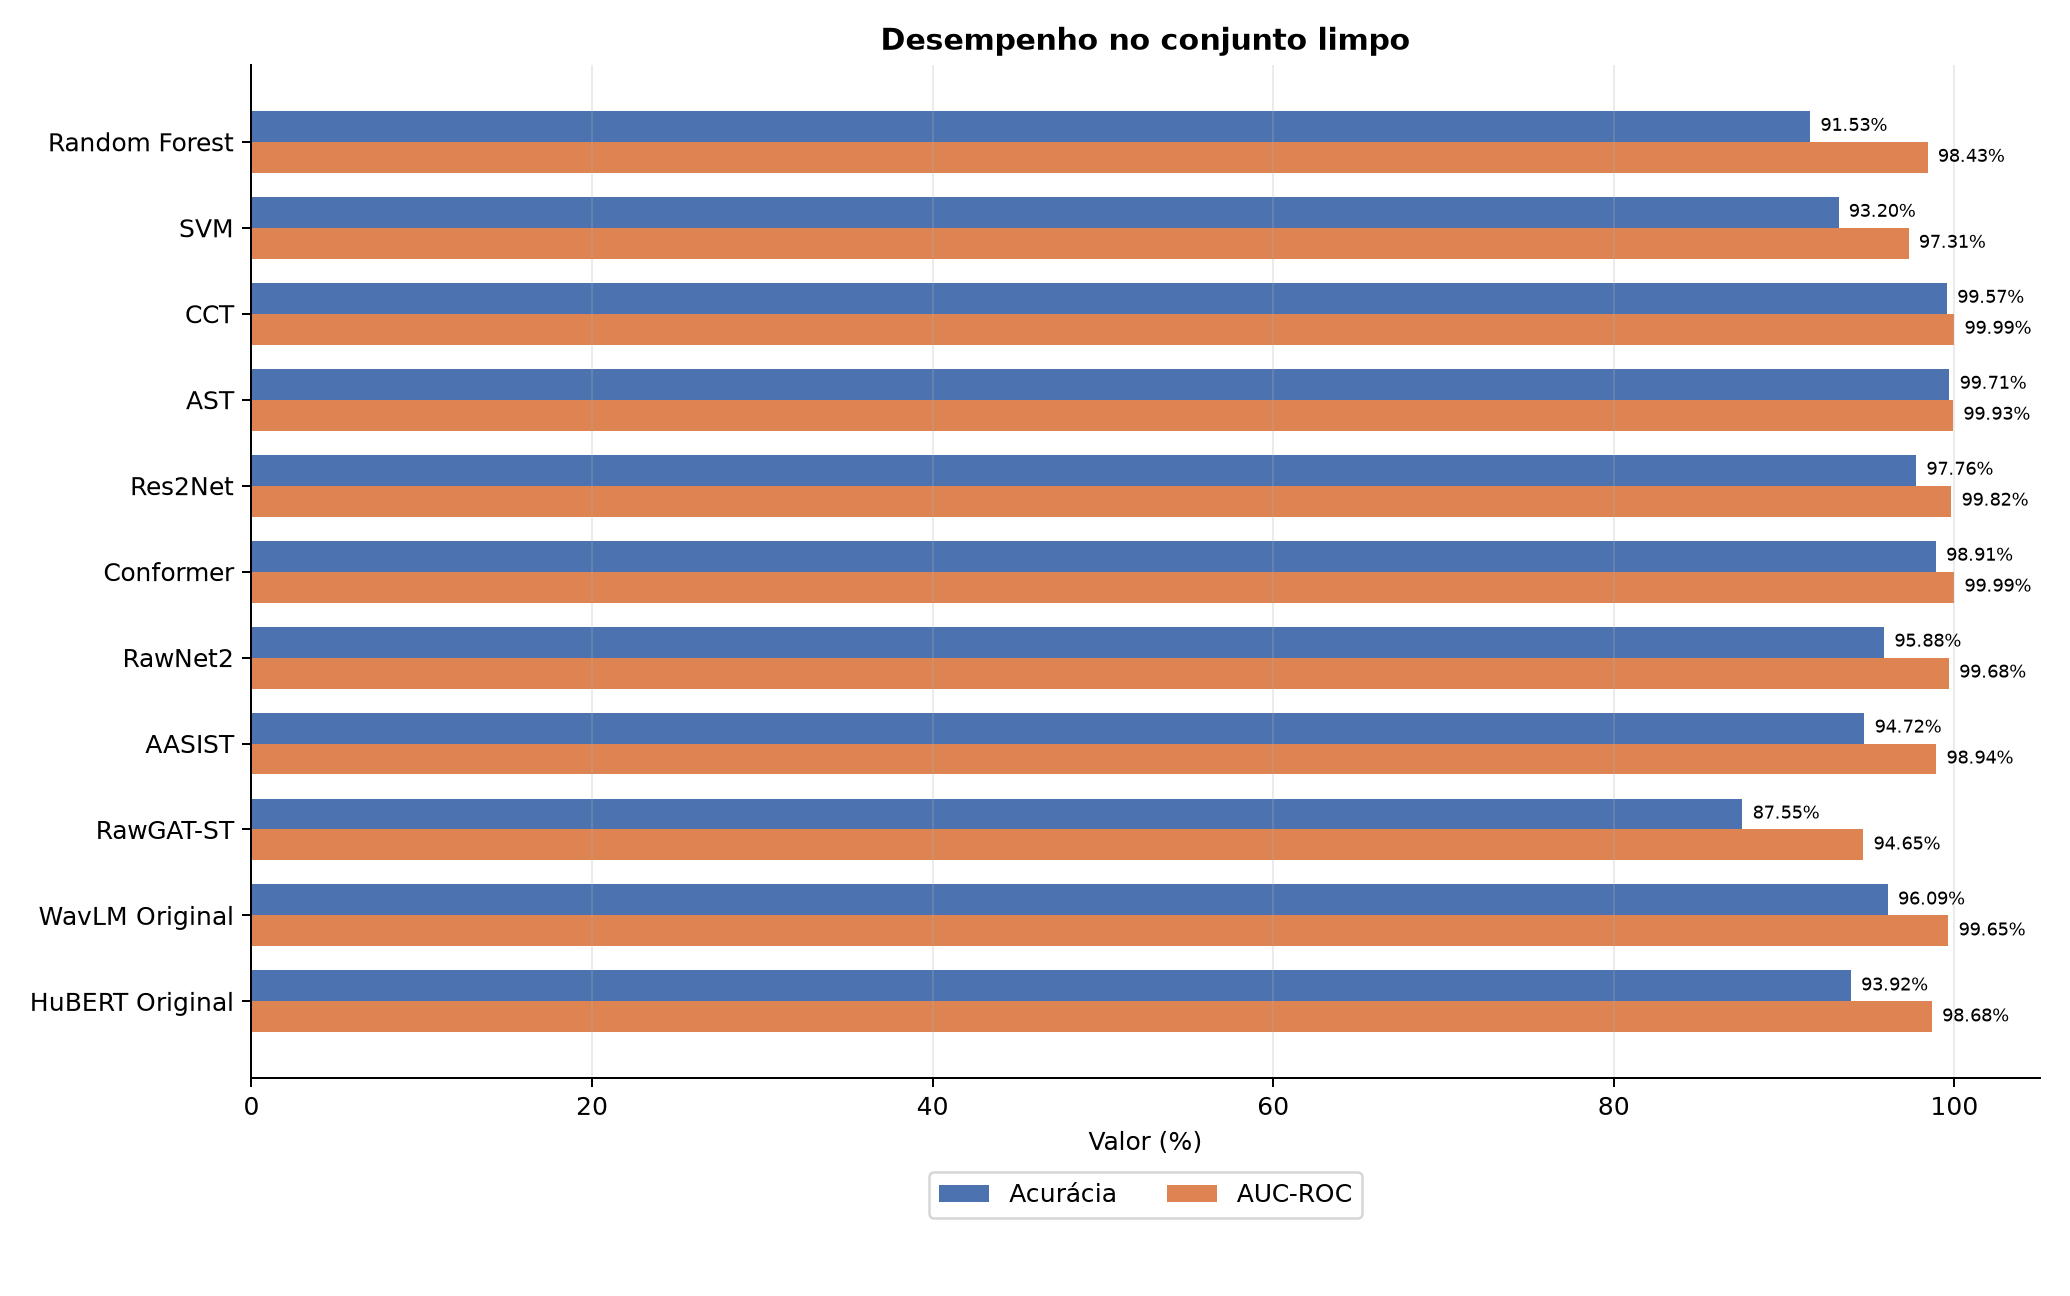
\includegraphics[width=\textwidth]{figures/benchmark_accuracy_auc.png}
\caption{Acurácia e AUC-ROC no conjunto de teste limpo.}
\label{fig:benchmark_accuracy_auc}
\end{figure}

\begin{figure}[ht]\centering

\includegraphics[width=\textwidth]{figures/benchmark_robustness.png}
\caption{Robustez a AWGN na forma de onda (acurácia vs.\ SNR).}
\label{fig:benchmark_robustness}
\end{figure}

\begin{figure}[ht]\centering

\includegraphics[width=0.92\textwidth]{figures/benchmark_eer.png}
\caption{Taxa de Erro Igual (EER) por arquitetura.}
\label{fig:benchmark_eer}
\end{figure}

\begin{figure}[ht]\centering

\includegraphics[width=0.92\textwidth]{figures/benchmark_tdcf.png}
\caption{$t$-DCF$^\ast$ por arquitetura.}
\label{fig:benchmark_tdcf}
\end{figure}

\begin{figure}[ht]\centering
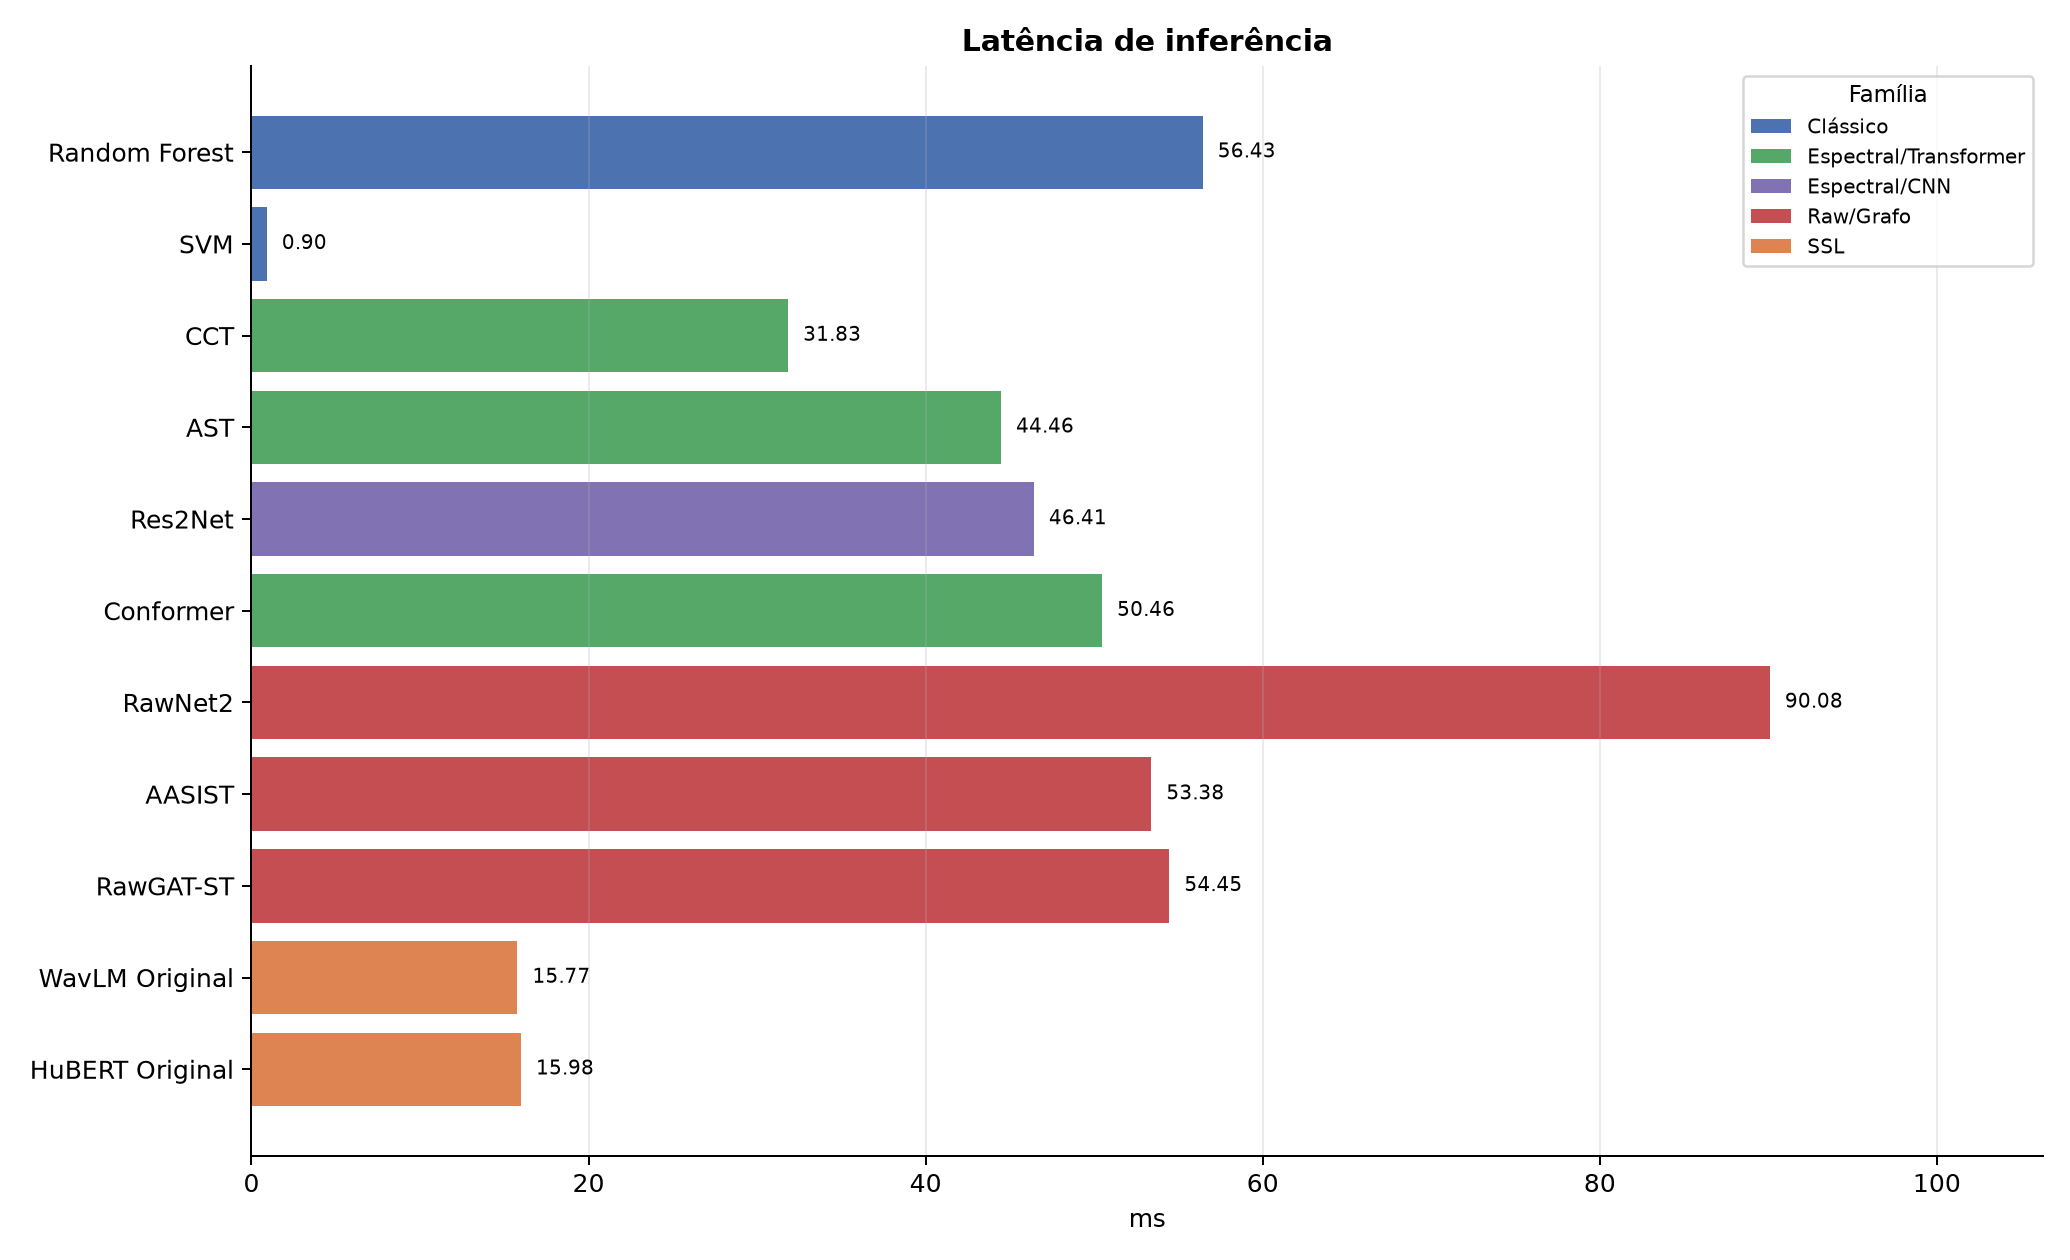
\includegraphics[width=0.95\textwidth]{figures/benchmark_latency.png}
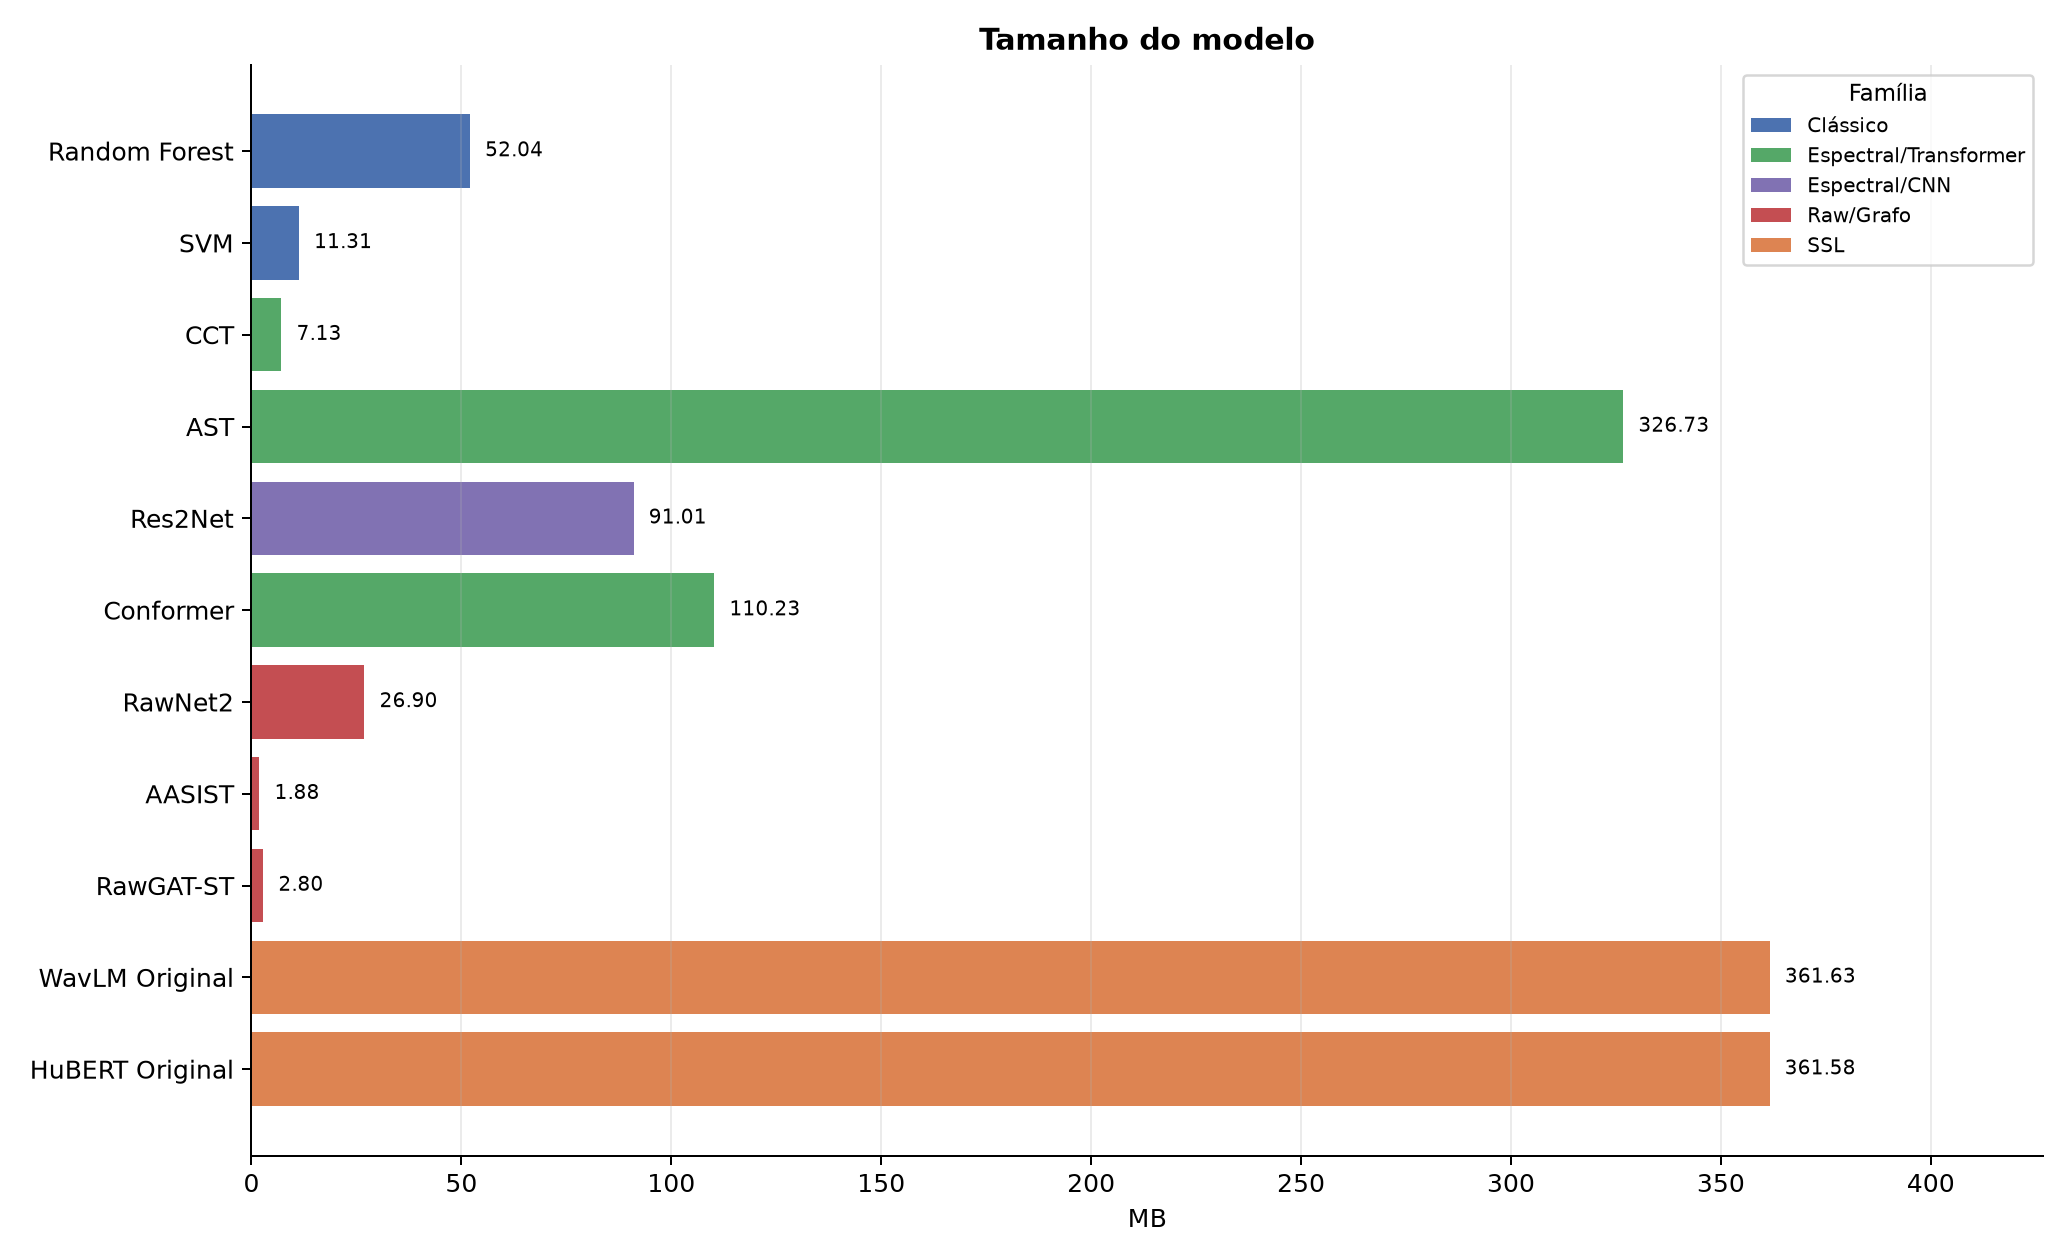
\includegraphics[width=0.95\textwidth]{figures/benchmark_size.png}
\caption{Latência e tamanho dos modelos.}
\label{fig:benchmark_latency_size}
\end{figure}

\begin{figure}[ht]\centering
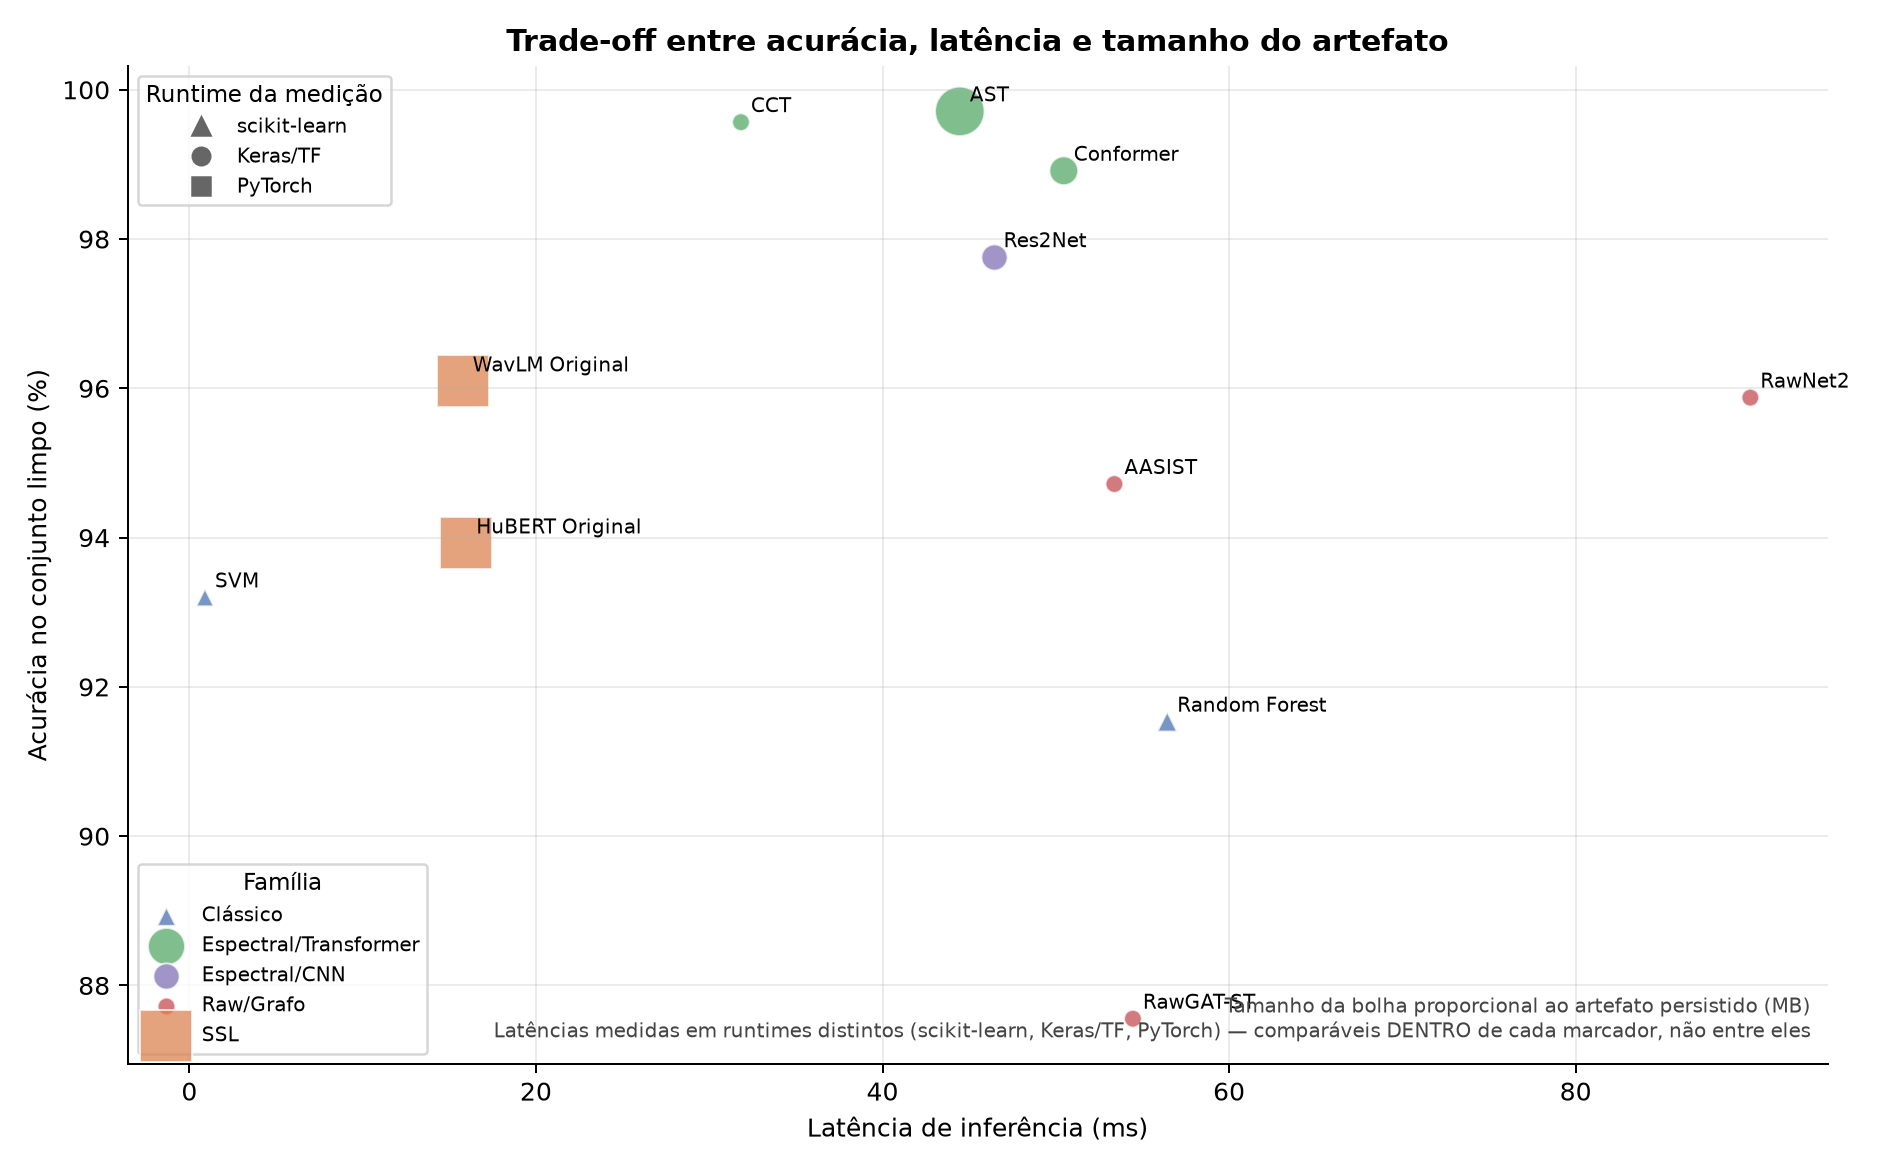
\includegraphics[width=0.95\textwidth]{figures/benchmark_accuracy_latency_tradeoff.png}
\caption{Trade-off entre acurácia, latência e tamanho dos artefatos.}
\label{fig:benchmark_accuracy_latency_tradeoff}
\end{figure}

\begin{figure}[ht]\centering
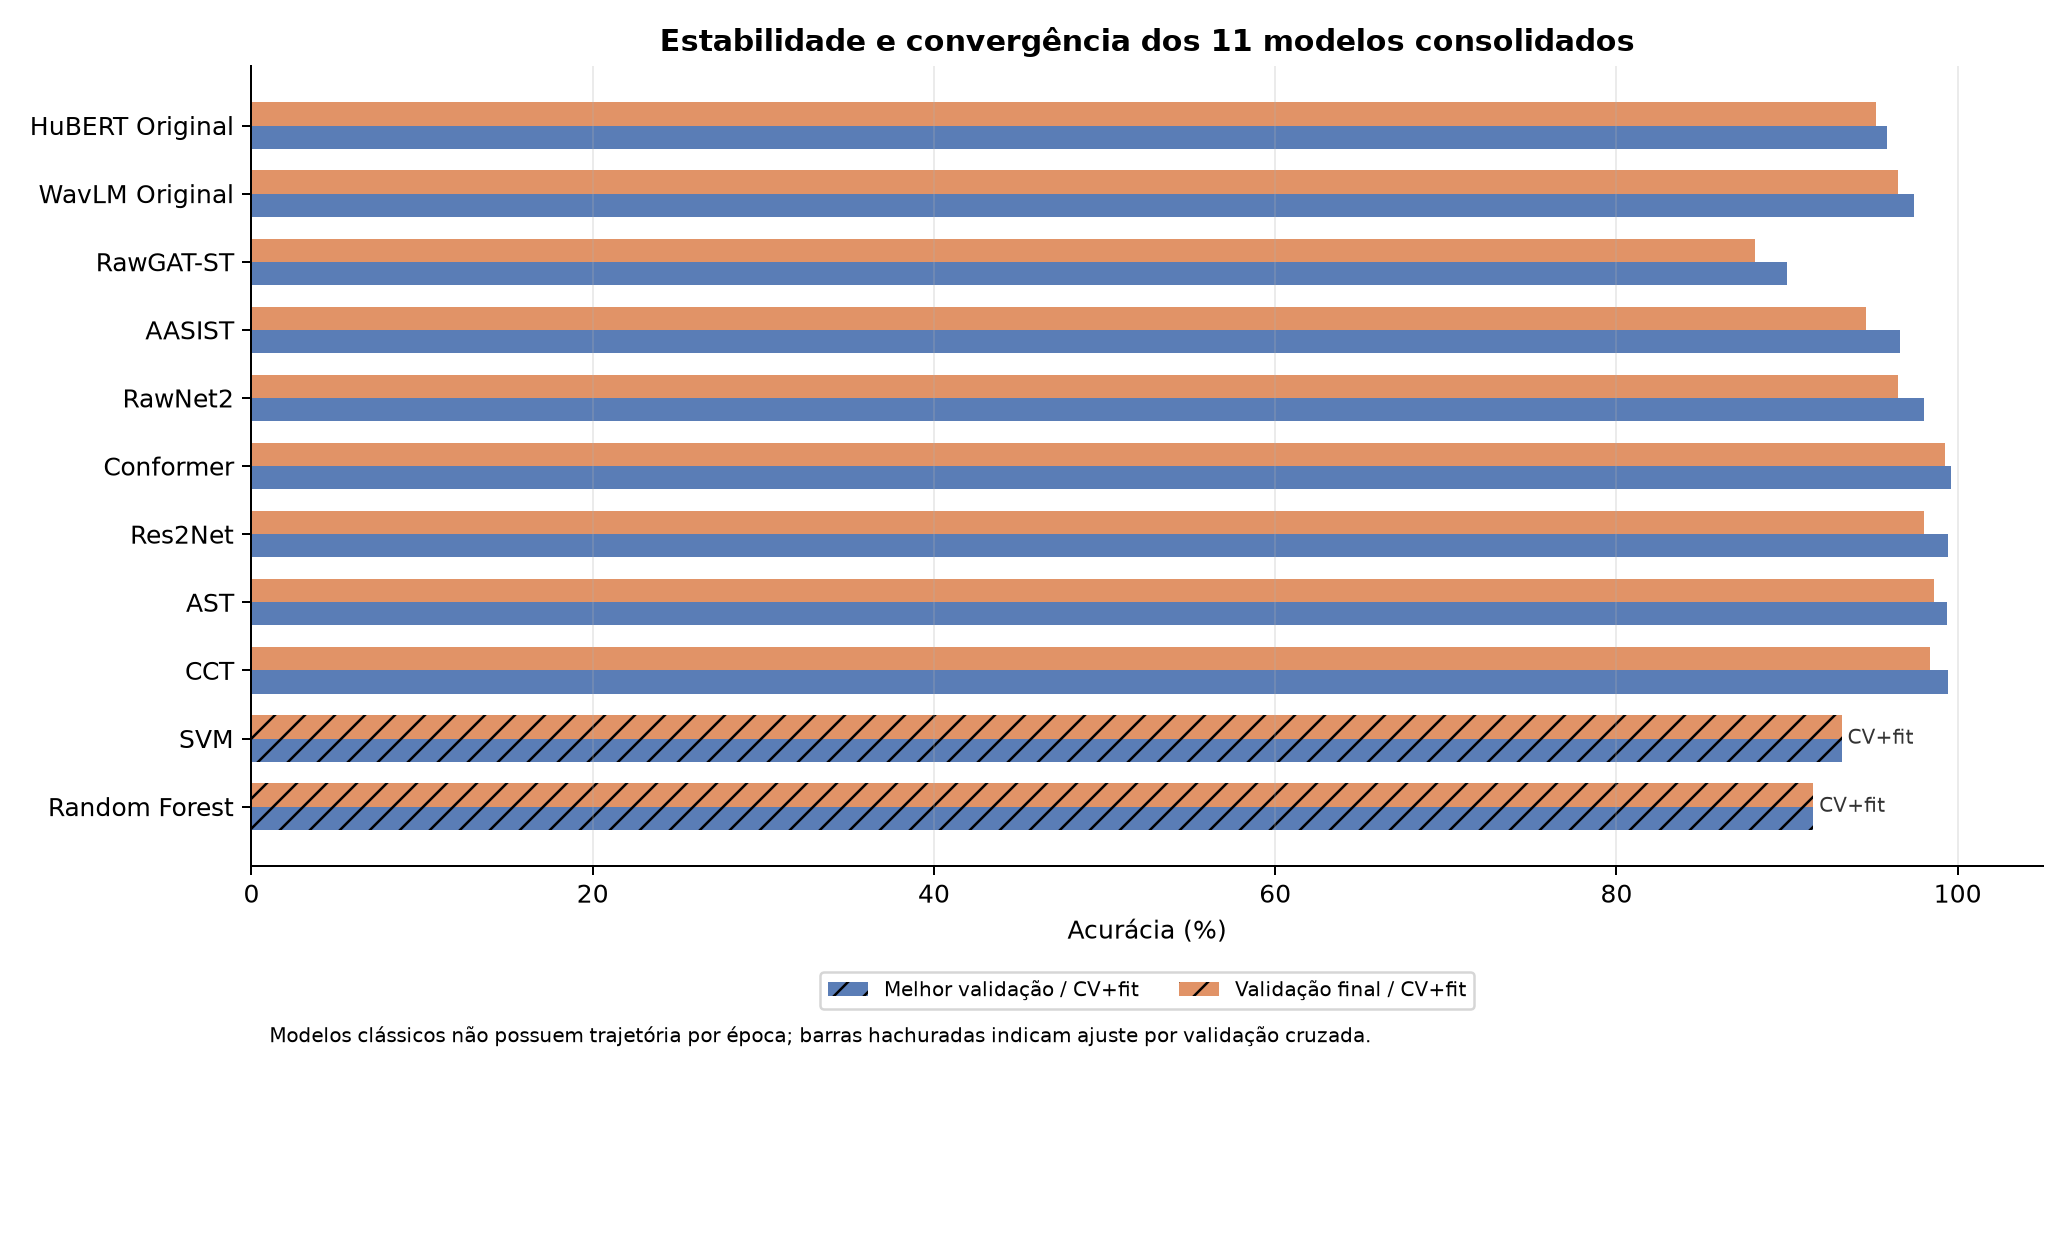
\includegraphics[width=0.95\textwidth]{figures/training_stability.png}
\caption{Resumo descritivo das curvas de validação em execução única; a diferença pico--final não demonstra, isoladamente, estabilidade de otimização. Modelos clássicos não possuem trajetória por época.}
\label{fig:training_stability}
\end{figure}

\begin{figure}[ht]\centering
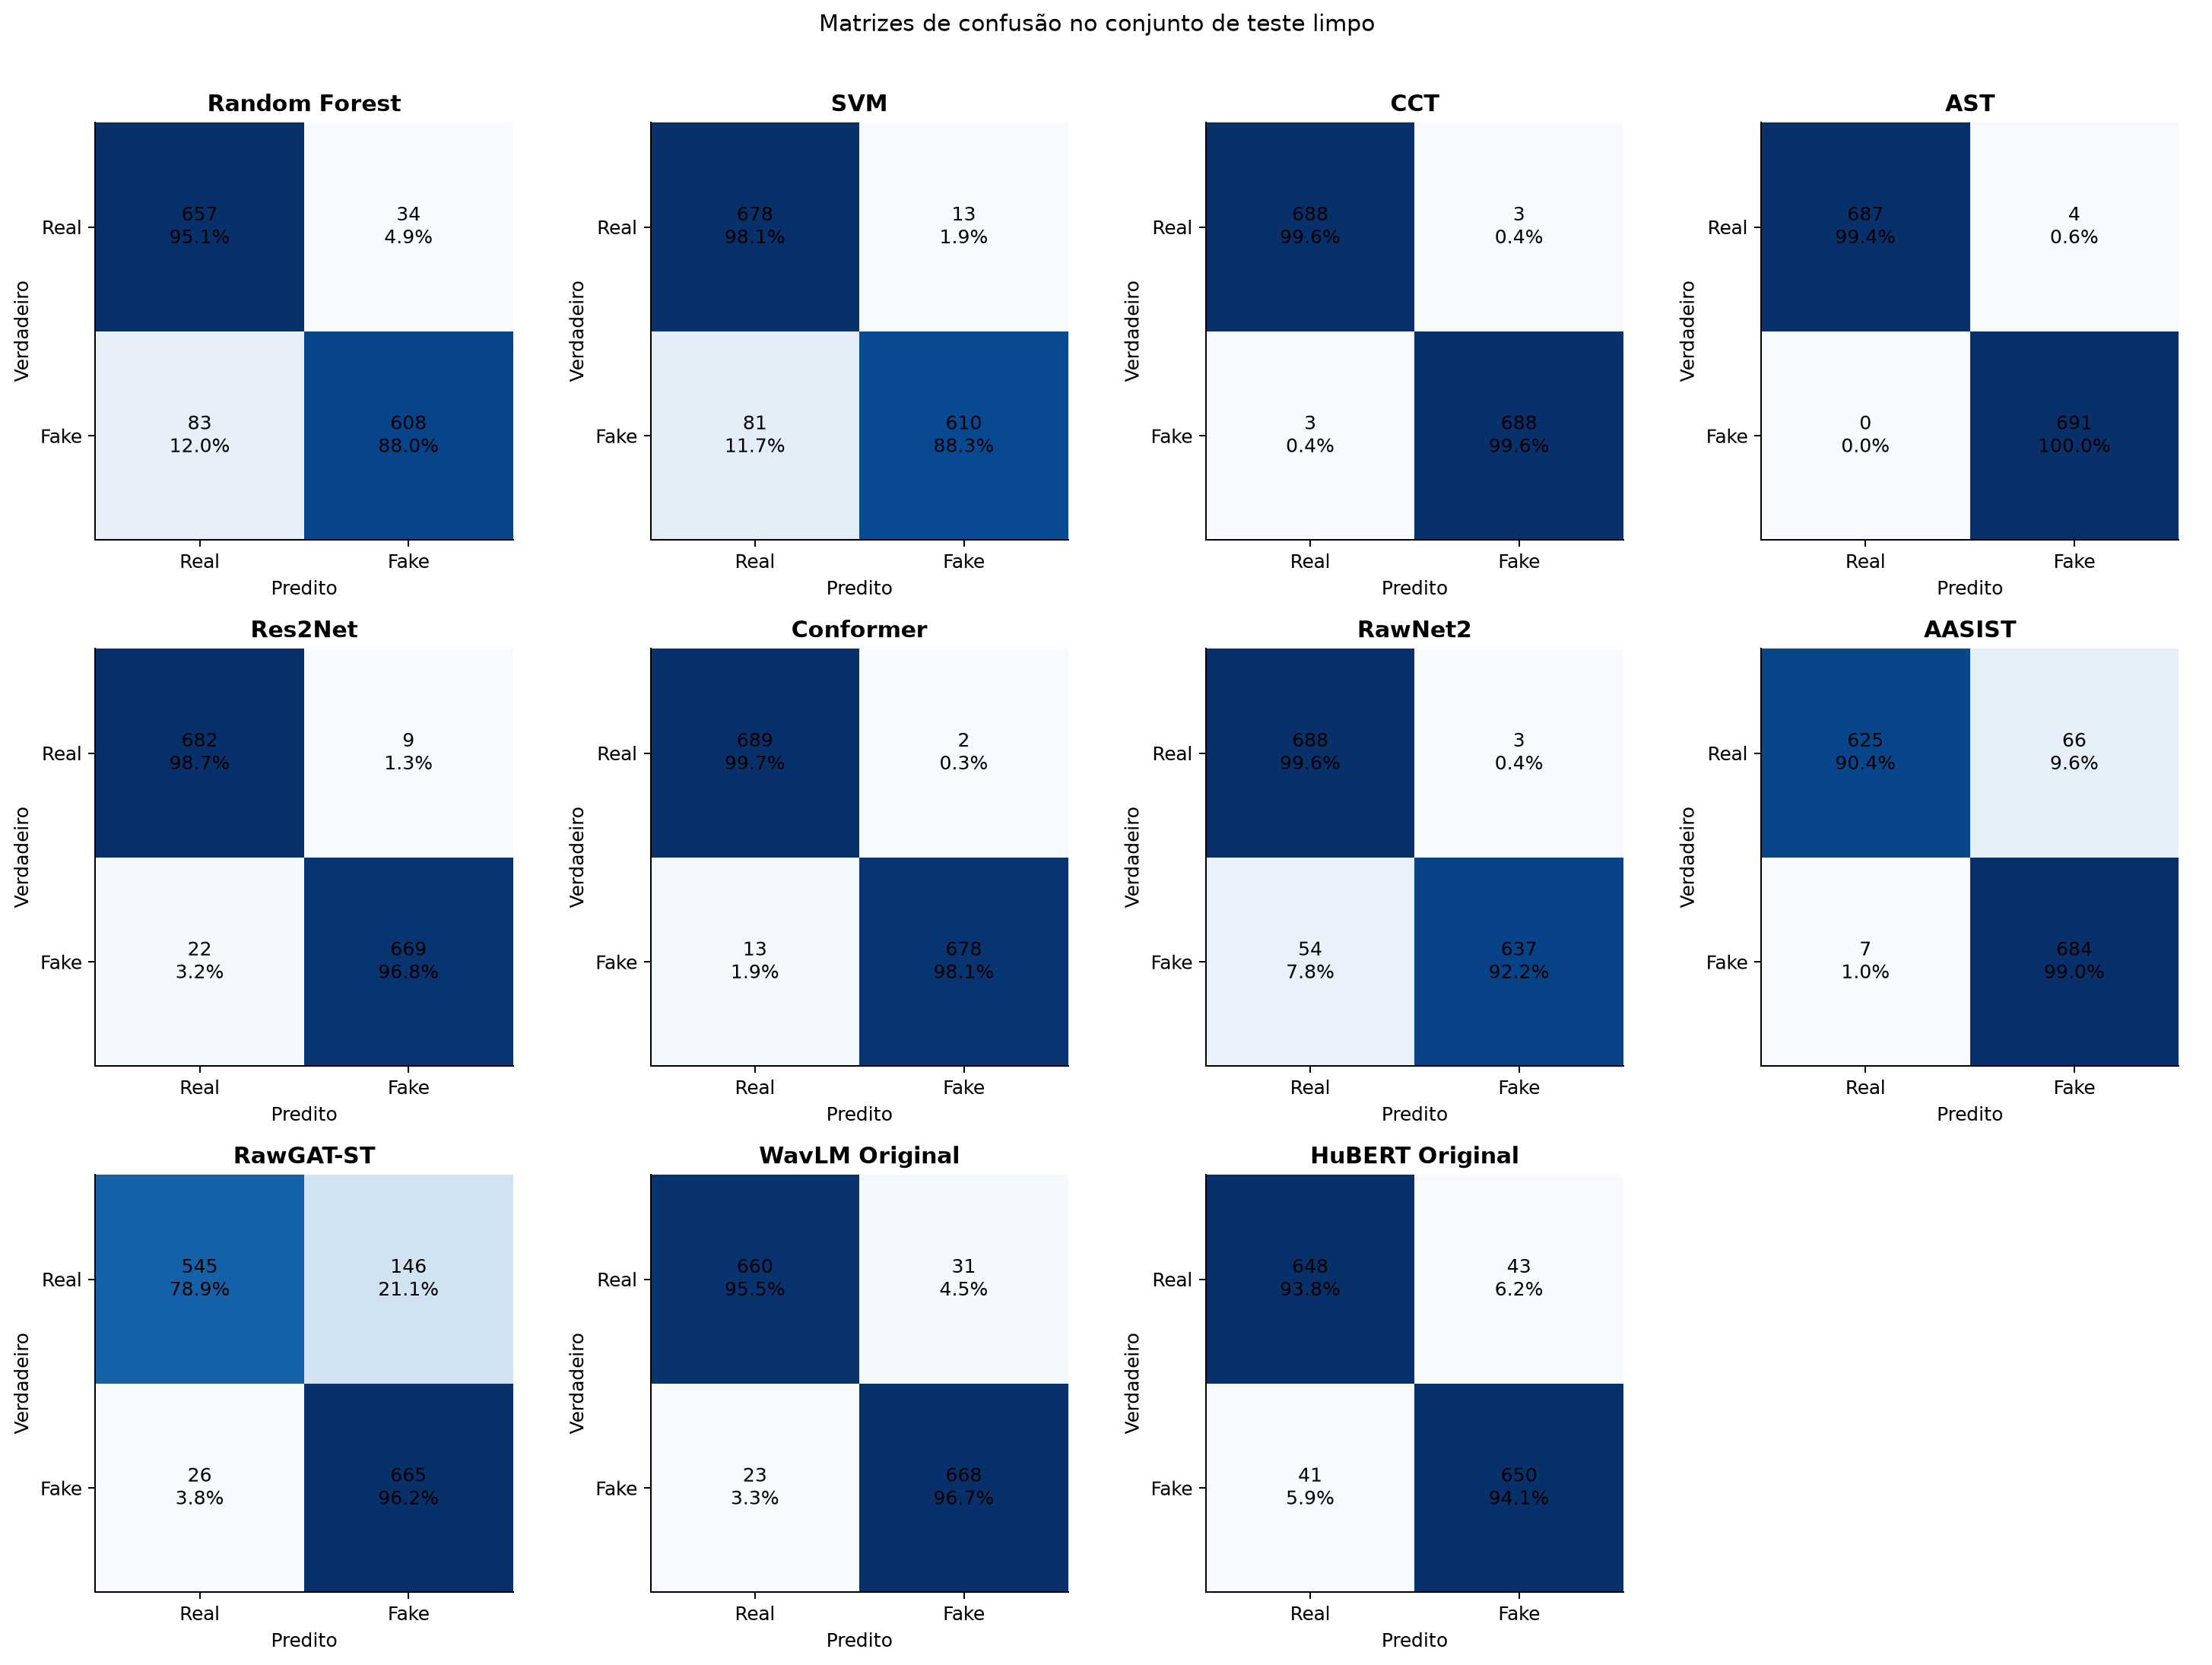
\includegraphics[width=\textwidth]{figures/confusion_matrices_article.png}
\caption{Matrizes de confusão dos onze modelos avaliados no artigo.}
\label{fig:confusion_matrices_article}
\end{figure}
